\documentclass[tikz,border=8pt]{standalone}
% Shared look for every TikZ diagram. Load with \input{../../tools/tikz-style.tex}
\usepackage[T1]{fontenc}
\usepackage{lmodern}
\renewcommand{\sfdefault}{lmr}  % diagrams use the same serif as the text
\usetikzlibrary{arrows.meta, positioning, shapes.geometric, calc, fit, backgrounds}
\definecolor{cblue}{HTML}{4C78A8}
\definecolor{corange}{HTML}{F58518}
\definecolor{cgreen}{HTML}{54A24B}
\definecolor{cred}{HTML}{E45756}
\definecolor{cpurple}{HTML}{B279A2}
\definecolor{cgrey}{HTML}{6B6B6B}
\tikzset{
  every picture/.style={font=\sffamily, line width=1.2pt},
  box/.style={draw=#1, fill=#1!12, rounded corners=4pt, align=center, inner sep=7pt, minimum height=1.1cm},
  box/.default=cgrey,
  arrow/.style={-{Stealth[length=3mm]}, draw=cgrey, line width=1.4pt},
  title/.style={font=\sffamily\bfseries\Large},
  note/.style={font=\sffamily\small, text=cgrey, align=center},
}
\AtBeginDocument{\hyphenpenalty=10000 \exhyphenpenalty=10000}

\begin{document}
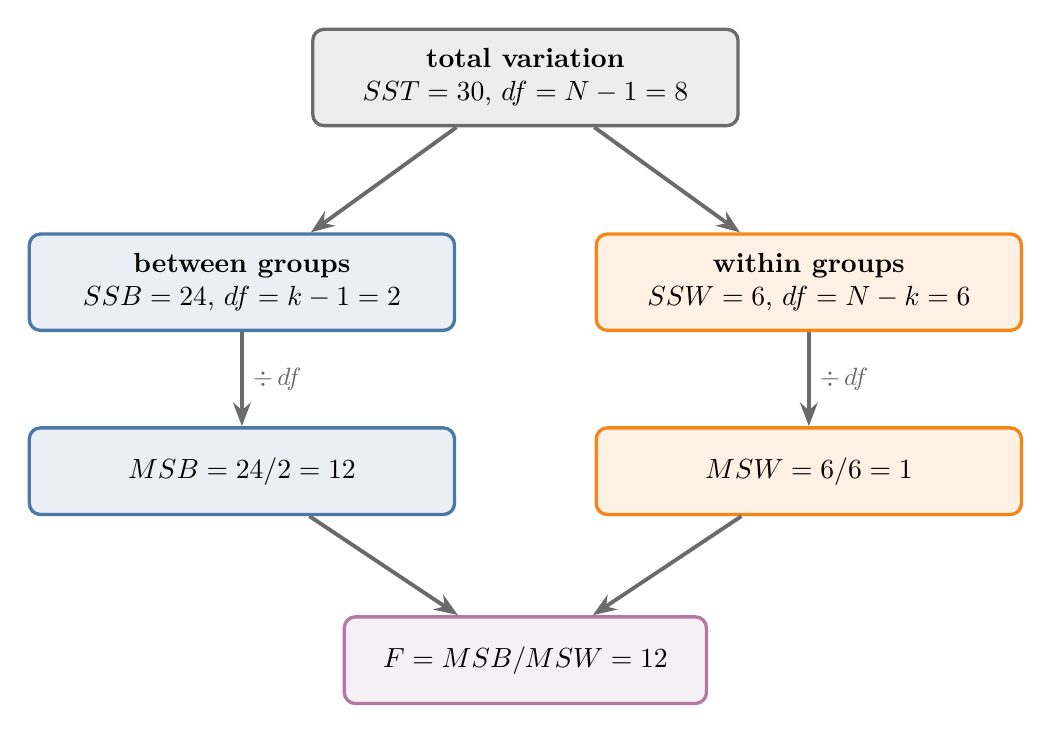
\begin{tikzpicture}
  \node[box=cgrey, minimum width=5.4cm] (t) at (0,0) {\textbf{total variation}\\ $SST = 30$, $df = N - 1 = 8$};
  \node[box=cblue, minimum width=5.4cm] (b) at (-3.6,-2.6) {\textbf{between groups}\\ $SSB = 24$, $df = k - 1 = 2$};
  \node[box=corange, minimum width=5.4cm] (w) at (3.6,-2.6) {\textbf{within groups}\\ $SSW = 6$, $df = N - k = 6$};
  \draw[arrow] (t) -- (b); \draw[arrow] (t) -- (w);
  \node[box=cblue, minimum width=5.4cm] (mb) at (-3.6,-5) {$MSB = 24 / 2 = 12$};
  \node[box=corange, minimum width=5.4cm] (mw) at (3.6,-5) {$MSW = 6 / 6 = 1$};
  \draw[arrow] (b) -- (mb) node[midway, right, note] {$\div\, df$};
  \draw[arrow] (w) -- (mw) node[midway, right, note] {$\div\, df$};
  \node[box=cpurple, minimum width=4.6cm] (f) at (0,-7.4) {$F = MSB / MSW = 12$};
  \draw[arrow] (mb) -- (f); \draw[arrow] (mw) -- (f);
\end{tikzpicture}
\end{document}
